\chapter{Preceding Work}
\label{cha:preceding}

Preceding to this bachelor thesis, a project seminar with the same title was taken. During this project seminar the first part of the project was implemented.

The outcome of this project seminar is described in the following chapter. A detailed description on how this was accomplished can be found in the respecting project report \cite{projectseminar}.
\\

\section{Hardware System}

\subsection{Architecture}

In this project a \gls{soc} was build on top of an \gls{fpga} using predefined \gls{ip} cores for the processor and additional system components.

An overview of the complete hardware architecture of the system described in the next sections is included in the appendix of the project seminar report (see \cite{projectseminar}, sec. A.1).
\\

\subsubsection{Processor}
\label{subsubsec:microblaze}

The used \textit{XC5VLX110T} \gls{fpga} does not have a build-in hard core processor, therefore a single core \textit{MicroBlaze} soft core processor was chosen. The \textit{MicroBlaze} processor is a proprietary processor, developed by \textit{Xilinx} for their \gls{fpga} families and supported by the Xilinx hard- and software development kits. Its design follows the Harvard architecture with separate data and instruction memory.

Running Linux kernel requires the presence of an \gls{mmu}. To improve the system performance instruction and data caches (16 KB), barrel shifter, multiplier (64 bit) and the hardware division modules were enabled.
\\

\subsubsection{Bus System}

For connecting the \textit{MicroBlaze} processor to other peripherals on the chip the \gls{plb}, invented by \textit{IBM} as part of the \textit{CoreConnect} bus system, was selected.

Prior to the \textit{Virtex-6} \gls{fpga} family, only this bus system was available. \textit{Virtex-6} \gls{fpga}s support also the \gls{axi} system, which is part of the \gls{amba}, designed by \textit{ARM}. The used \textit{Xilinx XC5VLX110T} \gls{fpga} is part of the \textit{Virtex-5} family, therefore \gls{plb} needed to be selected as interconnect type. \cite{axi_interconnect}[p. 1, facts table]
\\

\subsubsection{Memory}

The used evaluation board of type "\textit{XUPV5-LX110T}" contains a single-rank unregistered 256 MB DDR2 SODIMM, which is connected to the processor via a memory controller. This memory controller is implemented in the \textit{Multi-Port Memory Controller} (MPMC) \gls{ip} core. The memory base address was set to \texttt{0x50000000}.

\subsubsection{Network Interface}
\label{preceeding:net}

The \textit{Xilinx XC5VLX110T} \gls{fpga} has four \textit{Tri-Mode Ethernet Media Access Controllers}, designed to the IEEE 802.3-2002 specification, operating at 10, 100, and 1,000 Mb/s. \cite{virtex5}[p. 4, table 1] To use these hard core controllers an \texttt{xps\_ll\_temac} soft IP core was added to the \gls{soc}, acting as a wrapper for the hard core to integrate it into the system.


\gls{gmii} is a backwards compatible extension to \gls{mii} supporting data rates of up to 1,000 Mb/s. Therefore it was selected as physical interface type, because support for Gigabit Ethernet was desired, but there was no need for a reduced data path width. To enable correct operation mode using \gls{gmii} as physical interface type on the \textit{Xilinx XUPV5} board, the jumpers \texttt{J22} and \texttt{J23} need to be set to positions \texttt{1-2}.

Usage of an integrated checksum calculation circuit is enabled using the parameters \texttt{C\_TEMAC0\_TXCSUM} and \texttt{C\_TEMAC0\_RXCSUM}.

\subsection{Clocks}
\label{sec:clocks}

Clocks for the system are generated using a \textit{clock\_generator} \gls{ip} core with an external oscillator providing a 100 MHz clock. \cite{ug347}[p. 20]

Due to high delays on data paths in the decode pipeline stage, a clock period of at least \textit{9.12 ns} is required, resulting in a system clock frequency for the processor and local bus of 100 MHz.

The memory controller (MPMC) is driven by a base clock of 200 MHz, a clock with half the frequency of the base clock (100 MHz) and a 200 MHz clock signal, shifted by 90°. All these clock signals are controlled by the same \gls{pll} used by the system clock signal.

The \texttt{GTX\_CLK} port of the Ethernet \gls{mac} \gls{ip} core is driven by a clock signal with exactly 125 MHz for operating \textit{GMII} (defined by the specifications of GMII \cite{ieee802_3}[sec. 35.2.2.1]). For \gls{dma} and control logic, a clock signal with a frequency identical to the local bus clock is required. The \texttt{REFCLK} was connected to a 200 MHz clock, according to the respective manual of the \gls{ip} core \cite{xps_ll_temac}[p. 11, table 3].

\subsection{Endianness}

\begin{quote}
 "Endianness describes how multi-byte data is represented by a computer system and is dictated by the CPU architecture of the system." \cite{intel_endiannness}[p. 5]
\end{quote}

Architectures utilizing the little endian concept store the least significant byte (LSB) at the lowest address, in big endian architectures the most significant byte (MSB) is stored at the lowest address. \cite{intel_endiannness}[p. 6]

Linux can be build for little, as well as for big endian systems. Only confinement is that the used toolchain (compiler, etc. -- see \cite{projectseminar}[sec. 3.2.2]) needs to support the endianness of the architecture.

The \textit{MicroBlaze} processor has the parameter \texttt{C\_ENDIANNESS} to specify the endianness of the processor. But although the \textit{MicroBlaze Processor Reference Guide} states that "the \texttt{C\_ENDIANNESS} parameter is automatically set to little endian when using AXI4, and to big endian when using PLB, but can be overridden by the user" \cite{mb_ref}[p. 52], this parameter must not be changed for \textit{Virtex-5} \gls{fpga}s. This is reasoned in the disability of the peripheral cores connected via \gls{plb}, to handle data other than in big endian byte order. The \gls{axi} bus circumvents this problem by swapping bytes.\footnote{\url{http://forums.xilinx.com/t5/EDK-and-Platform-Studio/Memory-Test-fails-for-8-and-16-bit/m-p/253922/highlight/true\#M23973} (in-official statement by a Xilinx employee)}

Therefore big endian was selected for the system architecture of this project.

\clearpage
\section{Software}

\subsection{Linux Kernel}

\textit{Linux kernel} was chosen as the \gls{os} for the system. This is the pure core Linux \gls{os}, in comparison to enriched Linux distributions (like \textit{Ubuntu}, \textit{Debian}, \textit{openSUSE}, \textit{Fedora} and many more), which contain additional libraries, applications and configuration. The Linux kernel version used in this project contains further additions and bug fixes specific to the \textit{MicroBlaze} architecture by \textit{Xilinx}.

To enable correct recognition of the latest \textit{MicroBlaze} processor versions with enabled \gls{pvr}, it might be necessary to apply a patch included in the appendix of this report (\ref{subsec:pvr_patch}) to the Linux kernel sources. The patch was extracted from the \textit{PetaLogix} Linux kernel fork.

Building Linux kernel sources to an executable image file requires a set of tools (called toolchain) for compiling source code files and linking binary output to one single image. \textit{Xilinx} provides toolchains, based on the widely used \gls{gcc} and \textit{binutils}, for cross compiling from Linux x86 and x86-64 architectures to \textit{MicrobBlaze} systems as target architecture. Depending on the used development system, the corresponding toolchain has to be selected.
\\

\subsubsection{Configuration}

\begin{wrapfigure}{r}{.65\textwidth}
%	\begin{figure}[H]
	\centering
	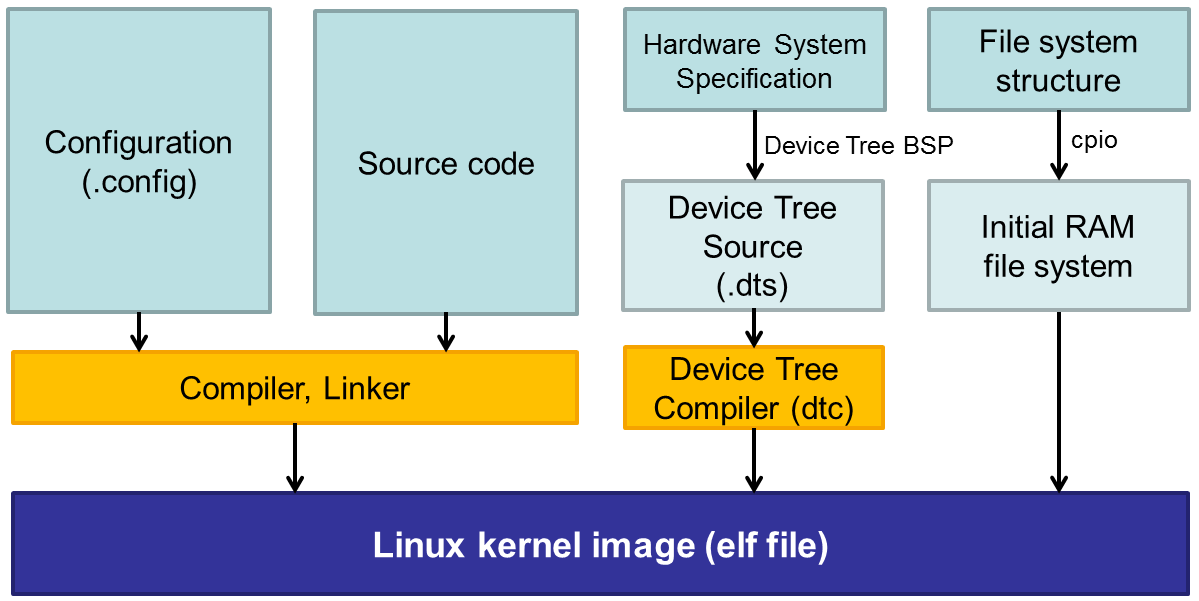
\includegraphics[width=.6\textwidth]{linux-config-build.png}
	\caption{Components of a Linux kernel build.}
%	\end{figure}
\end{wrapfigure}

Linux kernel consists of many optional sub-parts for target architectures, device drivers, special features, etc. Which of these parts are compiled and linked into the Linux kernel binary image needs to be configured in the \texttt{.config} file in the Linux kernel root directory. This file is "the configuration blueprint for building a Linux kernel image" \cite{linuxPrimer}[sec. 4.3.1] and contains all (required) settings.

The \textit{MicroBlaze} processor can be configured with different feature sets (multiplier, barrel shifter, etc.). Therefore the \gls{gcc} compiler needs to be parameterized for matching the provided features of the target system \cite{mb_linux}[sec. "Kernel Configuration Details"]. These need to be specified in the \texttt{XILINX\_MICROBLAZE0\_*} settings inside of the \texttt{.config} file. The \texttt{KERNEL\_BASE\_ADDR} is also an imported setting which must match the base address of the system's main memory.

The \texttt{XILINX\_LL\_TEMAC} driver is used for the Ethernet interface.

Another part of system configuration is the \textit{Device Tree}. It is an abstraction layer for accessing hardware information, to avoid compiling everything into architecture specific assembler code \cite{device_tree}. It is accessed by the Linux kernel during the boot process for configuring itself and on lookup of hardware information. Therefore the \textit{Device Tree Source (dts)} file is compiled by the \textit{Device Tree Compiler (dtc)} during the Linux kernel build process to an \textit{Device Tree Blob (dtb)} and linked into the final Linux kernel image. It can be generated using the \textit{Device Tree Generator}, a \gls{tcl} script reading a system specification file generated by \gls{xps}.
\\

\subsection{The File System}
\label{subsec:fs}

It is possible to use the Linux kernel without a file system, but the makes little sense in practical use. Therefore an \textit{Initial RAM Disk (initrd)} image is mounted as \textit{root file system (rootfs)} \cite{linuxPrimer}[sec. 6.1]. This is a file system packed into a \textit{cpio} archive and linked into the Linux kernel image. It is unpacked completely into the main memory during kernel boot process.
\\

\section{Deployment}

The generated \textit{bitstream} of the hardware system representing the \gls{soc}, needs to be programmed into the \gls{fpga} on every power-on. This is required, because the configuration of the \gls{fpga} being set by the \textit{bitstream} is volatile. Programming the \textit{bitstream} is straight forward and can be accomplished using the \textit{Xilinx iMPACT} tool, which is part of the \textit{Xilinx ISE Design Suite}.

When the Linux kernel build succeeded, the resulting \textit{\gls{elf}} file can be found at \texttt{arch/microblaze/boot/simpleImage.<dts-name>}. This file needs to be loaded into the \gls{fpga} using \textit{\gls{xmd}}, which is also part of the \textit{Xilinx ISE Design Suite}.

\chapter{Modifications to the System}

The preceding sections describe the state of the hardware and software system, at the end of the project seminar. Although the part of the project implemented during this bachelor thesis builds on top of the project seminar's outcome, some modifications needed to be made to these parts of the system. These modifications are described in the following sections.
\\

\section{Hardware}

Data and instruction caches were extended to 64 kilobytes. This gives a slight performance gain for the system, while the used \gls{fpga} had sufficient resources left.
\\

\section{Software}

The toolchain used during the preceding project was updated to the latest version provided by \textit{Xilinx}. This version has the identifier "\texttt{microblaze-unkwnown-linux-gnu-.... (crosstool-NG 1.14.1) 4.6.2 20111018 (prerelease)}". The \gls{gcc} version included in this version is \texttt{4.6.2}. This \gls{gcc} version is not compatible with the Linux kernel version used previously. Therefore the Linux kernel was updated to version 3.5.0 (commit \texttt{45b74487f57324fa66da40cd4d52be6f07e2aefd}\footnote{\url{http://git.xilinx.com/?p=linux-xlnx.git;a=commit;h=45b74487f57324fa66da40cd4d52be6f07e2aefd}}). The toolchain upgrade itself was required for the work on user space applications described in the following chapters.

The used web server software (nginx) requires the availability of an event module in the \gls{os}. Therefore \texttt{epoll} was activated in the Linux kernel configuration (\texttt{.config} file). This is done by setting the switch \texttt{CONFIG\_EPOLL=y}. Further explanations on this change can be found in the related chapter about the nginx architecture (see \ref{sec:nginx-arch}).

Another event, affecting the software part of this project was the corporate takeover of \textit{PetaLogix} by \textit{Xilinx} in late August 2012 \cite{takeover}. In consequence the efforts of both companies on Linux kernel development for the \textit{MicroBlaze} architecture were bundled, leading -- amongst others -- to a common source code repository for related developments. This alleviated working on the software part of the project.
\\

\section{The File System}

For deployment of user space applications to the test system a number of \textit{C standard library (libc)} components need to be copied to the system. This results in a combined Linux image size of about 25 MB. Loading this image into the \textit{MicroBlaze} memory using \gls{xmd} takes about 9 minutes. For frequent develop-deploy-test cycles this adds unnecessary burden to the overall development process.

To circumvent this problem during development on user space applications, the file system was embedded using \gls{nfs}. When using \gls{nfs}, a directory on another system is mounted as root file system on the \textit{MicroBlaze} system over the network.

To enable this change for the \textit{MicroBlaze} system, the Linux kernel configuration option \texttt{CONFIG\_CMDLINE} needs to be changed to the following value:

\texttt{CONFIG\_CMDLINE="console=ttyUL0 ip=192.168.2.125 rootfstype=nfs root=/dev/nfs rw $ \hookleftarrow$\\  nfsroot=192.168.2.112:/home/peschuster/customfs/complete,tcp"} %\swarrow\rhook

This sets \texttt{192.168.2.125} to be the static IP address, changes the root file system type to \gls{nfs}, connects to a \gls{nfs} server at another system with IP address \texttt{192.168.2.112} and mounts the directory \texttt{/home/peschuster/customfs/complete} as root file system with read and write permissions over TCP. It might be required to adjust the exact values for theses settings, depending on the current environment.

On the system hosting the mounted directory, \gls{nfs} server needs to be configured for allowing the respective directory to be mounted by the other system. On \textit{Debian} and \textit{Ubuntu} Linux distributions this is done by adding a line to "\texttt{/etc/exports}", which should look like the following: 

\texttt{/home/peschuster/project/customfs/complete	192.168.2.125(rw,sync,no\_root\_squash)}

This allows access to \texttt{/home/peschuster/project/customfs/complete} for mounting by a system with IP address \texttt{192.168.2.125} with read and write access and synchronous data transfer. The option \texttt{no\_root\_squash} allows access and modifications to files and directories belonging to the \texttt{root} user. It is required, because there are no users and user groups defined on the \textit{MicroBlaze} system.

For conducted performance tests in a later stage of this project, these temporary changes to file system mounting were reverted and the file system was embedded into the Linux kernel image as a packed \textit{cpio} archive.